
\chapter{Podstawy teoretyczne}
\section{Metaverse}


Termin Metaverse odnosi się do koncepcji hipotetycznej, zawsze włączonej sieci 3D wirtualnych przestrzeni w, których użytkownicy mogą wykonywać różnorodne czynności, takie jak kontakty towarzyskie, łączenie się w grupy, nauka, praca, zakupy i inne, dzięki wykorzystaniu opartych na danych i imersyjnych technologii \cite{smartcities5030043}\cite{metaverseDefinitionReview}. Jest to termin, który łączy w sobie koncepcje greckiego prefiksu „meta”, który oznacza „pełniejszy” lub „przekraczający”, oraz akronimu „Verse” oznaczającego „wszechświat”, który oznacza pojemnik czasoprzestrzenny. Idea metaversum została wprowadzona w powieści science fiction Neala Stephensona \definicja{Snow Crash} w 1992 roku. Szybki rozwój technologii takich jak blockchain, wirtualna (\english{Virtual Reality}) i rozszerzona (\english{Augmented Reality}) rzeczywistość, gry, sztuczna inteligencja i Internet Rzeczy \acronym{IoT} (\english{Internet Of Things}) sprawiły, że metaversum stała się jednym z najbardziej popularnych terminów w świecie technologii. Rozwiązania i usługi są opracowywane dla wirtualnych światów, aby umożliwić użytkownikom dobrą zabawę, inteligentne angażowanie się w otoczenie i nawiązywanie głębszych relacji z innymi użytkownikami \cite{metaverseAsAService}. 

\begin{figure}[htbp!]
    \centering
    \includesvg[width=0.7\textwidth]{images/metaverse/MetaverseInfographic.svg}
    \caption{Koncepcyjny widok metaverse\cite{metaverseUseCaseslee}}
    \label{fig:enter-label}
\end{figure}

Metaverse działa jako połączony ze sobą wirtualny wszechświat, płynnie integrując się ze światem fizycznym poprzez dane i mechanizmy informacji zwrotnej, jednocześnie wchodząc w interakcje z różnymi ludzkimi działaniami, takimi jak rozrywka, edukacja i interakcje rodzinne, wspierane przez zaawansowane technologie, takie jak \akronim{AI} (\english{Artificial intelligence}), XR i blockchain. Interakcja ta została przedstawiona na rys.\ref{abstractMetaverseArchitectureHumanVirtualPhisical}. Metaverse jest uważany za idealne ucieleśnienie Internetu w przyszłości. Zintegrowany z zaawansowanymi technologiami, metaversum może być wirtualną przestrzenią wzbogaconą o rzeczywistość fizyczną. Użytkownicy są połączeni w wirtualnym wszechświecie w immersyjnej interakcji i są ze sobą połączeni w celu prowadzenia działań społecznych. Odkąd koncepcja metaversum została zaproponowana w powieści \definicja{Snow Crash}, ludzie się stopniowo przyzwyczajają do wirtualnych i internetowych aktywności zamiast fizycznych i konwencjonalnych. Ponadto, jako nowy paradygmat produkcji, produkcja w chmurze zapewnia użytkownikom usługi na żądanie w intuicyjny i wygodny sposób. Rozproszone zasoby produkcyjne są wirtualizowane i zarządzane w ujednolicony, zoptymalizowany i konfigurowalny sposób, umożliwiając wysoce wirtualną współpracę i innowacyjną produkcję\cite{industrialMetaverseForSmartManufacturing}. 

\begin{figure}[htbp!]
    \centering
    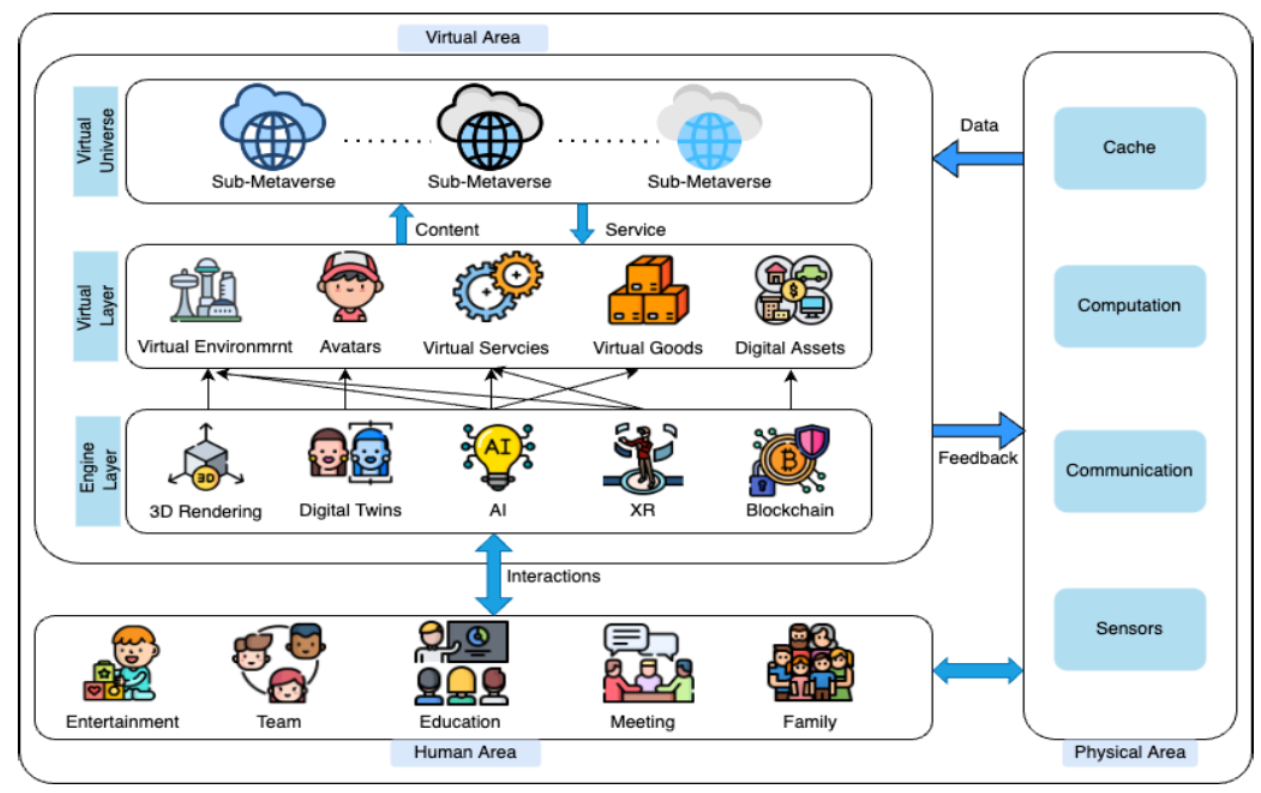
\includegraphics[width=\textwidth]{images/metaverse/metaverseAbstractArchitecture.png}
    \caption{Interakcje w architekturze Metaverse\cite{aSurveyofMobileEdgeComputingForMetaverse}}
    \label{abstractMetaverseArchitectureHumanVirtualPhisical}
\end{figure}

Kluczowe cechy Metaverse:

\begin{itemize}
    \item Trwałość:  oznacza, istnienie niezależnie od fizycznej obecności użytkownika\cite{metaverseAFullDive}.
    \item Nieskończoność: obsługiwanie niezliczonej liczby użytkowników i światów VR\cite{metaverseAFullDive}.
    \item Samowystarczalność: oznacza, że użytkownicy mogą zarabiać w Metaverse i płacić za swoją użyteczność\cite{metaverseAFullDive}.
    \item Interoperacyjność: pomaga użytkownikom przenosić ich wirtualne przedmioty, w tym awatary, z jednego projektu Metaverse do drugiego\cite{metaverseAFullDive}.
    \item Czas rzeczywisty: pozwala użytkownikom cieszyć się doświadczeniami w czasie rzeczywistym\cite{metaverseAFullDive}.
\end{itemize}


Metaverse ma być imersyjnym wirtualnym światem, który płynnie łączy sferę fizyczną i cyfrową, umożliwiając użytkownikom interakcję, współpracę i angażowanie się w szereg działań we wspólnym wirtualnym środowisku. U podstaw tej rewolucyjnej koncepcji leży niezawodna infrastruktura, która służy jako szkielet, ułatwiając łączność i interoperacyjność. Infrastruktura Metaverse to ewoluująca, złożona sieć wzajemnie połączonych technologii, protokołów i frameworków, które współpracują ze sobą w celu stworzenia jednolitego i spójnego wirtualnego wszechświata\cite{metaverseInfrastructureIEEE}.

Infrastruktura ta obejmuje szeroką gamę komponentów, w tym szybkie sieci, wydajne, o dużej mocy zasoby obliczeniowe, zaawansowane urządzenia sprzętowe i najnowocześniejsze platformy oprogramowania. Wykorzystuje ona najnowsze osiągnięcia w takich dziedzinach jak rzeczywistość wirtualna, rzeczywistość rozszerzona, blockchain i zdecentralizowane przetwarzanie danych, aby zapewnić immersyjne i bezpieczne doświadczenia korzystania z metaversum użytkownikom na całym świecie\cite{metaverseInfrastructureIEEE}.

\subsubsection{Architektura sieci w metaversum}

Architektura sieci w Metaverse została zaprojektowana tak, aby wspierać bezproblemowe interakcje i komunikację w czasie rzeczywistym, umożliwiając użytkownikom angażowanie się w różne działania bez doświadczania opóźnień lub rozłączeń. Wykorzystuje ona zaawansowane protokoły i technologie sieciowe, które priorytetowo traktują niskie opóźnienia, wysoką przepustowość i wydajny transfer danych\cite{metaverseInfrastructureIEEE}.

Zdecentralizowane sieci odgrywają kluczową rolę w zwiększaniu łączności Metaverse. Wykorzystując technologię blockchain i sieci peer-to-peer, infrastruktura Metaverse ma na celu zmniejszenie zapotrzebowania na centralne władze lub pośredników. Władze centralne, takie jak organy rządowe, duże korporacje lub scentralizowane platformy, kontrolują i regulują operacje w systemie, podczas gdy pośrednicy, tacy jak podmioty przetwarzające płatności, brokerzy danych lub dostawcy usług, ułatwiają transakcje lub interakcje między użytkownikami. Minimalizując zależność od tych podmiotów, Metaverse sprzyja bardziej otwartemu i sterowanemu przez użytkowników ekosystemowi. Takie podejście zwiększa odporność poprzez dystrybucję danych i usług w wielu węzłach, zmniejszając ryzyko pojedynczego punktu awarii i zapewniając, że Metaverse pozostaje funkcjonalne i dostępne, nawet jeśli części sieci zostaną wyłączone. Przejrzystość jest osiągana dzięki zastosowaniu technologii blockchain, która zapewnia przejrzystą księgę transakcji i działań, budując zaufanie wśród użytkowników, którzy mogą weryfikować działania i upewnić się, że nie ma ukrytych programów lub manipulacji. Demokratyczne zarządzanie pozwala użytkownikom uczestniczyć w rozwoju i procesach decyzyjnych Metaverse, umożliwiając im głosowanie nad propozycjami, sugerowanie zmian i wspólne kształtowanie kierunku wirtualnego świata, dając im poczucie własności i zaangażowania w jego ewolucję\cite{metaverseInfrastructureIEEE}.

Przesyłanie danych i zarządzanie nimi w ramach infrastruktury Metaverse jest ułatwione dzięki połączeniu tradycyjnych technologii sieciowych i nowych systemów rozproszonych, które obejmują technologię blockchain, zdecentralizowane rozwiązania pamięci masowej i protokoły sieciowe peer-to-peer. Szybkie sieci światłowodowe i łączność bezprzewodowa 5G/6G zapewniają przepustowość niezbędną do przesyłania informacji zawierających dużo treści multimedialnych i strumieni danych w czasie rzeczywistym. Jednocześnie zdecentralizowane rozwiązania pamięci masowej, takie jak rozproszone systemy plików i InterPlanetary File System \akronim{IPFS}, zapewniają bezpieczne i redundantne przechowywanie danych, umożliwiając efektywny dostęp do zasobów cyfrowych i ich wyszukiwania\cite{metaverseInfrastructureIEEE}.

Technologie przetwarzania na krawędzi (\english{Edge Computing}) mogą znacząco przyczynić się do zwiększenia wydajności infrastruktury metaversum. Przenosząc obliczenia i przetwarzanie bliżej urządzeń brzegowych (takich jak zestawy VR i okulary AR), przetwarzanie brzegowe zmniejsza opóźnienia i poprawia szybkość reakcji, zapewniając płynniejsze, bardziej immersyjne i wysoce interaktywne wrażenia użytkownika. Podejście to odciąża również scentralizowane serwery od zadań przetwarzania, rozkładając obciążenie obliczeniowe na całą sieć i zapewniając skalowalność w miarę wzrostu rozmiaru i złożoności metaversum\cite{metaverseInfrastructureIEEE}.

Technologia blockchain może odgrywać kluczową rolę w zwiększaniu bezpieczeństwa sieci w metaversum. Wykorzystując zdecentralizowane mechanizmy konsensusu i protokoły kryptograficzne, blockchain zapewnia integralność i niezmienność danych, chroniąc przed manipulacją i nieautoryzowanym dostępem. Dodatkowo, inteligentne kontrakty ułatwiają bezpieczne i przejrzyste interakcje, automatycznie wykonując wcześniej zdefiniowane umowy zapewniając w ten sposób wszystkim stronom możliwość niezależnej weryfikacji wyników. Umożliwia to transakcje bez zaufania, w których uczestnicy mogą prowadzić wymianę bez konieczności ufania sobie nawzajem lub centralnemu organowi, usprawniając złożone procesy w architekturze Metaverse i modelowaniu 3D.\cite{metaverseInfrastructureIEEE}.

\subsubsection{Wymagania sprzętowe metaversum}

Aby uzyskać dostęp i w pełni doświadczyć funkcjonalności oferowanych przez metaversum, użytkownicy będą potrzebować specjalistycznego sprzętu, który może obsługiwać immersyjne środowiska wirtualne i interakcje takie jak rozpoznawanie gestów w czasie rzeczywistym i precyzyjne śledzenie ruchu. Podstawą tych wymagań sprzętowych są urządzenia komputerowe, takie jak komputery stacjonarne, konsole do gier lub wyspecjalizowane stacje robocze do rozwoju Metaverse. Urządzenia te muszą posiadać wystarczającą moc obliczeniową, możliwości graficzne i zasoby pamięci, aby renderować szczegółowe środowiska 3D i obsługiwać złożone symulacje w technologii Metaverse\cite{metaverseInfrastructureIEEE}.

Infrastruktura Metaverse w dużym stopniu wykorzystuje urządzenia rzeczywistości rozszerzonej i wirtualnej, aby zapewnić użytkownikom immersyjne wrażenia. Zestawy VR, takie jak Oculus Rift, HTC Vive i PlayStation VR, przenoszą użytkowników do w pełni zrealizowanych wirtualnych światów, umożliwiając im interakcję z cyfrowymi obiektami i awatarami tak, jakby były prawdziwe. Urządzenia AR, takie jak Microsoft HoloLens i Magic Leap One, efektywnie łączą elementy cyfrowe ze światem fizycznym, umożliwiając użytkownikom rozszerzenie otoczenia o wirtualne nakładki i interaktywne interfejsy\cite{metaverseInfrastructureIEEE}.

Zaawansowane jednostki przetwarzające, w tym wysokowydajne procesory graficzne \akronim{GPU} (\english{Graphics Processing Unit}) i wyspecjalizowane akceleratory, odgrywają kluczową rolę w zwiększaniu doznań płynących z Metaverse. Komponenty te są odpowiedzialne za renderowanie złożonych środowisk 3D, dokładne symulowanie zjawisk fizycznych, takich jak dynamika płynów i kolizje, a także przetwarzanie ogromnych ilości danych w czasie rzeczywistym. Dodatkowo, integracja sztucznej inteligencji i technologii uczenia maszynowego w infrastrukturze Metaverse wymaga potężnych zasobów obliczeniowych, aby umożliwić inteligentne interakcje, przetwarzanie języka naturalnego i realistyczne awatary\cite{metaverseInfrastructureIEEE}.

Wraz z ciągłym rozwojem technologii, infrastruktura Metaverse wykorzystuje nowe technologie, które mogą jeszcze bardziej poprawić wrażenia użytkownika. Przykładowo, rozwój interfejsów mózg-komputer \akronim{BCI} (\english{Brain-Computer Interface}) i pozwala na korzystanie z urządzeń dotykowych, które odzwierciedlają zachowanie urządzenia wirtualnego w świecie rzeczywistym. Te technologie mogą zrewolucjonizować sposób interakcji użytkowników ze środowiskami wirtualnymi, umożliwiając bardziej intuicyjne i immersyjne doświadczenia. Co więcej, postępy w dziedzinie obliczeń kwantowych i przetwarzania fotonicznego znacznie zwiększy moc obliczeniową i możliwości przetwarzania danych w metaversum, umożliwiając bardziej złożone symulacje, analizy w czasie rzeczywistym i zaawansowane interakcje oparte na sztucznej inteligencji.\cite{metaverseInfrastructureIEEE}.

\subsubsection{Transakcje w metaversum}

Wirtualne waluty i technologia blockchain znajdują się w czołówce, jeśli chodzi o ułatwianie transakcji w Metaverse. Te cyfrowe aktywa, często określane jako kryptowaluty lub tokeny, mogą służyć jako podstawowy środek wymiany towarów, usług i wirtualnych aktywów w wirtualnym środowisku Metaverse. Wykorzystując zdecentralizowany i bezpieczny charakter technologii blockchain, te wirtualne waluty umożliwiają płynne, przejrzyste transakcje, eliminując potrzebę pośredników i zmniejszając koszty transakcji\cite{metaverseInfrastructureIEEE}.

Inteligentne kontrakty, które są samowykonywalnymi umowami zakodowanymi w sieciach blockchain, mogą odgrywać kluczową rolę w automatyzacji i zabezpieczaniu transakcji w Metaverse. Kontrakty te definiują zasady i warunki różnych umów, takich jak transfery aktywów, umowy o świadczenie usług i rozliczenia finansowe. Po wdrożeniu, inteligentne kontrakty wykonują się automatycznie, gdy spełnione są wcześniej określone warunki, zapewniając przejrzystość, wydajność i niezmienne prowadzenie dokumentacji dla wszystkich transakcji w ramach immersyjnego doświadczenia Metaverse\cite{metaverseInfrastructureIEEE}.

Prawa własności wirtualnej są kolejnym obszarem, który wymaga starannego rozważenia w ramach zarządzania i regulacji Metaverse. Ponieważ użytkownicy inwestują w wirtualne nieruchomości, aktywa cyfrowe i własność intelektualną, taką jak sztuka cyfrowa, muzyka i oprogramowanie, kluczowe znaczenie ma posiadanie dobrze zdefiniowanych zasad i mechanizmów ustanawiania i ochrony tych praw. Może to obejmować integrację rozwiązań opartych na technologii blockchain i zdecentralizowanych rozwiązań w zakresie przechowywania. Tokeny niewymienialne \akronim{NFT} (\english{Non-Fungible Token}) mogą być wykorzystywane do reprezentowania tych unikalnych zasobów cyfrowych. Tokeny te są przechowywane w sieciach blockchain, zapewniając łatwą weryfikację własności i pochodzenia. Ponadto zdecentralizowane systemy przechowywania plików, takie jak IPFS, umożliwiają bezpieczne i redundantne przechowywanie treści cyfrowych, zapewniając długowieczność i dostępność wirtualnych zasobów\cite{metaverseInfrastructureIEEE}.

Infrastruktura Metaverse może usprawnić wirtualne rynki i interakcje gospodarcze poprzez integrację zdecentralizowanych aplikacji \akronim{dApps} (\english{Decentralized application}) i zdecentralizowanych protokołów finansowych \akronim{DeFi} (\english{decentralized finance}). Platformy te umożliwiają użytkownikom kupowanie, sprzedawanie, handlowanie i inwestowanie w szeroką gamę wirtualnych aktywów, towarów i usług. Inteligentne kontrakty automatyzują i zarządzają tymi transakcjami, zapewniając uczciwość, przejrzystość i przestrzeganie wcześniej określonych zasad. Co więcej, zdecentralizowane autonomiczne organizacje \akronim{DAO} (\english{Decentralized autonomous organization}) pozwalają na zbiorowe podejmowanie decyzji i zarządzanie w ramach tych wirtualnych rynków, wspierając poczucie wspólnoty i współwłasności\cite{metaverseInfrastructureIEEE}.

\subsubsection{Ekosystem Metaverse}

\begin{figure}[!htbp]
    \centering
    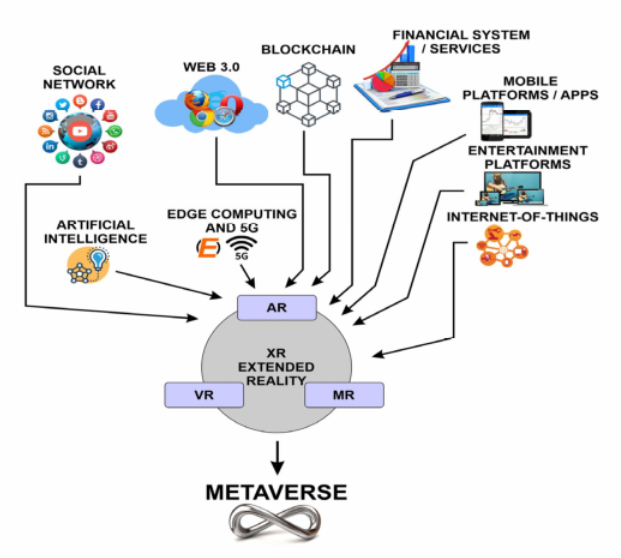
\includegraphics[width=\textwidth]{images/metaverse/metaverseEcosystem.png}
    \caption{Ekosystem Metaverse\cite{metaverseSecurityIssuesChallengesAndViableZTAModel}}
    \label{metaverseEcosystemImage}
\end{figure}

Metaverse umożliwia realizację kilku nowatorskich scenariuszy biznesowych w wielu różnych branżach. Rys.\ref{metaverseEcosystemImage} przedstawia nadrzędny ekosystem technologiczny umożliwiający powstanie metaversum. Nie ulega wątpliwości, że technologie AR/VR/MR i XR stanowią podstawę metaversum, umożliwiając użytkownikom dostęp do wirtualnego świata 3D. W swojej najwcześniejszej iteracji Metaverse może być zbiorem aplikacji Web 3.0 zapewniającym ograniczone wrażenia VR. W kontekście Metaverse, Web 3.0 oferuje kilka kluczowych funkcji. Wykorzystuje technologię blockchain do tworzenia zdecentralizowanych platform, zmniejszając zależność od centralnych władz i pośredników, zwiększając w ten sposób bezpieczeństwo i zaufanie. Standardy Web 3.0 ułatwiają integrację i interakcję między różnymi aplikacjami i platformami w ramach Metaverse, umożliwiając spójne i ujednolicone środowisko wirtualne. Oczekuje się, że sieci społecznościowe będą jednymi z pierwszych, które przeniosą się do Metaverse, umożliwiając użytkownikom udostępnianie i konsumowanie treści immersyjnych. Technologia blockchain zostanie szeroko wdrożona w Metaverse, aby umożliwić realizację wizji zdecentralizowanych finansów i gospodarki twórców, które są nowymi tematami, głównie ze względu na bezpieczeństwo i prywatność, które oferują. Aplikacje i platformy mobilne mogą być kolejnymi, które migrują do Metaverse, a następnie platformy rozrywkowe. Wreszcie, łączność \akronim{5G/6G}, oferująca niskie opóźnienia, może być spoiwem, które płynnie połączy wszystkie elementy, podczas gdy Internet Rzeczy będzie łączył wszystkie urządzenia wraz z intensywnym wykorzystaniem sztucznej inteligencji, w tym inteligencji brzegowej, w celu zapewnienia spersonalizowanych doświadczeń\cite{metaverseSecurityIssuesChallengesAndViableZTAModel}.


Można przewidzieć, że ekosystem Metaverse przedstawiony na rys.\ref{metaverseEcosystemImage} może przyjąć trzy potencjalne ścieżki ewolucji:

\begin{itemize}
    \item Zamknięty Metaverse: Dla niszowych aplikacji i przypadków użycia ograniczonych do użytku przez konkretną społeczność o wyspecjalizowanych potrzebach.
    \item Federacyjny: Zarządzana i obsługiwana przez dużą korporację z ekosystemem współpracujących partnerów, zewnętrznych dostawców i usługodawców dostarczających użytkownikom końcowym ujednolicone doświadczenie.
    \item Otwarty Metaverse: Metaversum niesfederowana, nie kontrolowana przez żaden pojedynczy podmiot. O otwartej architekturze i społeczności deweloperów tworzących aplikacje/usługi dla użytkowników końcowych.
\end{itemize}



Prawdopodobnym jest, że ekosystem Metaverse, jak przedstawiono na rys.\ref{metaverseEcosystemImage}, może przyjąć trzy formy. Można oczekiwać, że wszystkie trzy modele będą współistnieć w takiej czy innej formie. Rozwiązanie Meta oferowane przez firmę Facebook jest doskonałym przykładem modelu federacyjnego\cite{metaverseSecurityIssuesChallengesAndViableZTAModel}. 

Oczekuje się, że w przyszłości pojawią się inne modele, głównie tworzone przez konsorcja tworzące strategiczne sojusze biznesowe, fuzje korporacyjne i przejęcia. Jest prawdopodobne, że Metaverse napotka kilka przeszkód na drodze do jego szerokiego przyjęcia. Niektóre z wyzwań stojących na drodze do realizacji pełnego potencjału koncepcji Metaverse i jej przyjęcia obejmują:

\begin{itemize}
    \item Dostęp: Obecnie tylko przez zestawy okularów wirtualnej rzeczywistości, które nie są aktualnie powszechne
    \item Łatwość użytkowania: Użytkownicy uważają, że obecna wersja zestawów okularów wirtualnej rzeczywistości jest nieporęczna i trudna do noszenia przez długi czas
    \item Brak rozwiniętego ekosystemu: Niewiele aplikacji dostępnych na obecnych platformach VR
    \item Bezpieczeństwo i prywatność: Środowiska XR cierpią z powodu luk w zabezpieczeniach podstawowych technologii, w tym kwestii dotyczących prywatności użytkowników w wirtualnych światach. 
\end{itemize}

Podczas gdy oczekuje się, że postęp technologiczny rozwiąże kwestie dostępu i łatwości użytkowania w najbliższej przyszłości, kwestie bezpieczeństwa i prywatności muszą być budowane od podstaw podczas projektowania ekosystemu Metaverse\cite{metaverseSecurityIssuesChallengesAndViableZTAModel}.